\chapter{Workshop results}
\label{WorkshopResults}
As it is elaborated on in \autoref{ChapterWorkshop}, the purpose of the card sort and workshop is to elicit mental models of the users' interaction with a TonePrint community platform. In the workshop this is investigated for two specific tasks, which on their own don't provide a full explanation for how the entire information architecture should be. The given tasks are the overall new features going from the current TonePrint app to a TonePrint community, and the results are as such also overall explanations. For further elaborating explanations, the various elements in each task should be investigated on their own as a set of subtasks. The subjects' mental models are derived from their hand drawn concept maps and subsequent explanations of them, which was video recorded, and the purpose of the following chapter is to present the results of this workshop before uniting them with the results of the card sort.

\section{The individual task}
\label{IndividualTaskResults}
The workshop was conducted in a meeting room at TC Electronic's headquarters in Aarhus, and five members of their staff served as subjects for this. It's important to note that none of them have been affiliated with either the development or maintenance of the TonePrint application at any point, so they were considered fitting subjects for the workshop. The obvious bias of including developers of the TonePrint app would have meant that the workshop wouldn't have produced mental models representing those of the end-users. One of the subjects, however, was considered a potential bias as he develops templates for User TonePrints. He has not had any influence on the design of the TonePrint app though, so he was included in the individual task any way but instead served as an observer for the group task, leaving the remaining four subjects for this.

For the individual task, the results produced five different hand drawn concept maps, these are all found in \autoref{App:WorkshopConceptMaps}. The results for the subjects are presented individually including their concept map, depicted with software to make it more presentable and readable, a table of their highlighted content and actions, and codings of their video presentations. For the depicting of the concept maps it was considered insufficient to create a complete remake of their drawings alone, as they differ greatly in terms of structure and detail. In order to balance these differences, the new concept maps are made from their presentation of their drawings. The major pieces of content such as sites, list etc. are depicted in rectangles, while the components within this content, such as search, filtering etc. are depicted in rounded rectangles. The connections and actions between these elements are depicted as pointers. The codings of their explanations are presented with the concept map with the important content and actions highlighted with \textbf{bold text}. This is done to put the content and actions into context and not only have them displayed in a table.

\subsection*{Subject 1}
\label{Subject1}
Subject 1 starts from the \textbf{TonePrint app} where he wants to \textbf{Log in} in case he isn't already. Then he enters his \textbf{my TonePrints site} which contains a tab either called \textbf{friends}, \textbf{community} or something more fitting. He presses this tab and is redirected to either a \textbf{search friends} functionality or simply a \textbf{friends list}. The two could also be combined to include the search functionality within the friends list. He uses the search functionality by writing \textbf{user 1}, so it is the only name in the list, and by pressing the username he enters his \textbf{profile}. On this profile he is presented a \textbf{list of TonePrints} created by user 1. The list is divided into the tabs \textbf{by name} and \textbf{by type}. From the list of types, he selects the \textbf{Corona TonePrints} and under this he wants to select \textbf{Warm Corona}. This selection could either be confirmed by an \textbf{add to my list} option or a button with a gear symbol on it, even though he's not completely sure what would happen by pressing it. Instead he proposes pressing the name of the TonePrint which would unveil a heart, giving him the choice of \textbf{liking} the TonePrint. It would also present him with instructions in the shape of \textbf{about}, \textbf{how i use it}, and \textbf{number of users}.\\
%
\begin{table}[H]
\begin{minipage}[b]{\linewidth}\centering
	\begin{tabular} {|l|l|l|} \hline
		\rowcolor{xGray25} \textbf{Content and Components} & \textbf{Actions} \\  \hline
		TonePrint app & Logging in \\
		My TonePrints site & Pressing friends/community tab \\
		Friends/Community tab & Writing "user 1" \\
		Search functionality & Pressing user 1 name \\
		Friends list & Filter by type \\
		User 1 profile & Selecting Warm Corona \\
		List of TonePrints & Pressing "add to my TonePrints" \\
		Type and name filter & Pressing like functionality \\
		Corona TonePrints & \\
		Warm Corona & \\
		Like functionality & \\
		About this TonePrint & \\
		How i use this TonePrint & \\
		Number of users & \\ \hline
	\end{tabular}
	\caption{The important content, components, and actions mentioned by subject 1}
	\label{tab:Subject1ContentActions}
\end{minipage}
\end{table}
%
\begin{figure}[H]
	\centering
	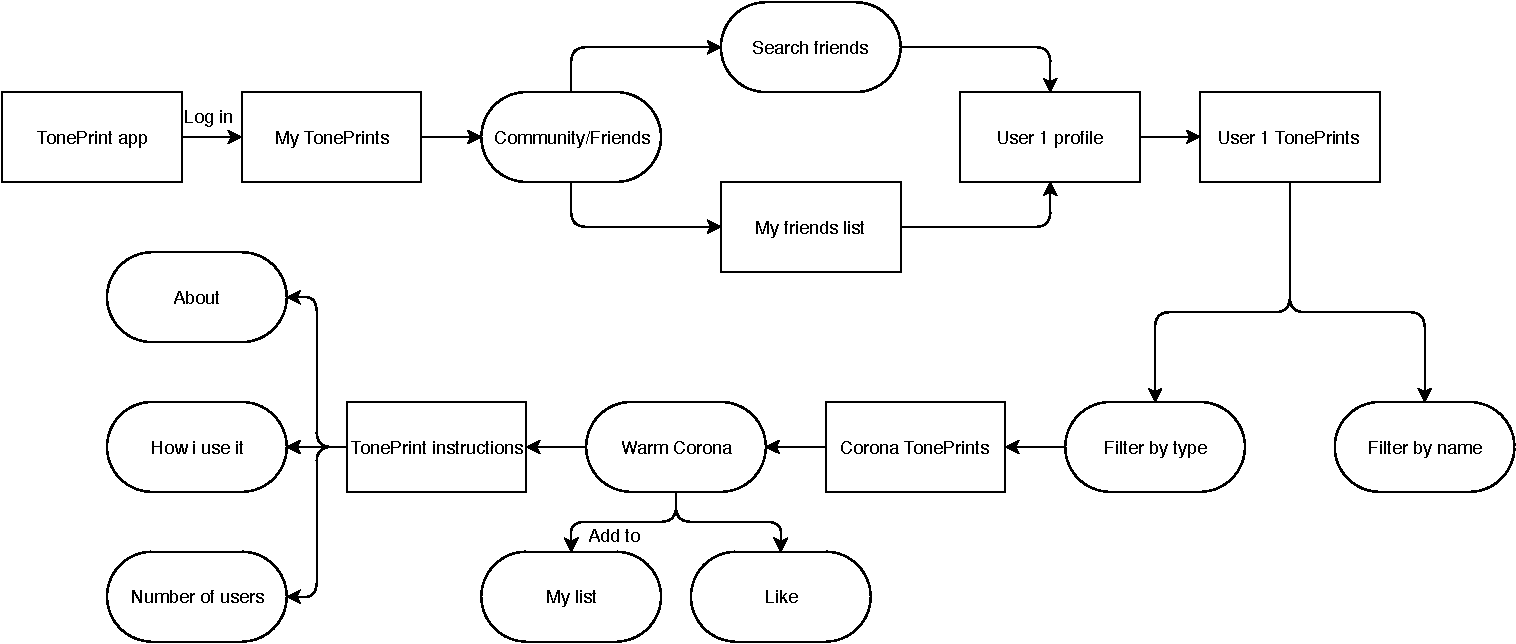
\includegraphics[width=0.95\textwidth]{1ICMM_new.pdf}
	\caption{The concept map for subject 1. The hand-drawn map is displayed in \autoref{fig:DrawnICMM1}.}
	\label{fig:ICMM1}
\end{figure}


\subsection*{Subject 2}
\label{Subject2}
Subject 2 starts by opening the \textbf{TonePrint app}, after this he has two options. The user can either open his list of \textbf{subscriptions}, if he's looking for a user that he already has subscribed to, or he can open another \textbf{list} and simply \textbf{search} for user 1. Whatever the approach, the next step is then to hook up a pedal and guitar, and select one of \textbf{user 1's Corona TonePrints}. He selects one of them and \textbf{Loads it to his pedal}. Subject 2 then tries out the TonePrint by playing the guitar, and if doesn't like it, he goes back and selects a new TonePrint. If he does like the TonePrint, he wants to \textbf{highlight} it as one of his \textbf{favourites}, so he can find it at another time. He would also like to \textbf{store it in his pedal}. Finally, by selecting to subscribe to the user, he would expect the system to send him \textbf{notifications}, when the user uploads \textbf{new TonePrints}, either directly in the app or maybe by mail. When all these steps are clear, subject 2 would then expect to unhook the pedal from the app and start playing with the TonePrint in question. \\
%
\begin{table}[H]
\begin{minipage}[b]{\linewidth}\centering
	\begin{tabular} {|l|l|l|} \hline
		\rowcolor{xGray25} \textbf{Content and Components} & \textbf{Actions} \\  \hline
		TonePrint app & Looking through "subscribed to" users \\
		Subscriptions list & Searching for user 1 \\
		Search list & Hook up pedal and guitar \\
		User 1 Corona TonePrints list & Selecting a user 1 TonePrint \\
		Favourites list & Loading TonePrint to pedal \\
		Notifications of new TonePrints & Trying out the TonePrint \\
		 & Highlight as favourite \\
		 & Storing TonePrint in pedal \\
		 & Unhook pedal from the app \\ \hline
	\end{tabular}
	\caption{The important content, components, and actions mentioned by subject 2}
	\label{tab:Subject2ContentActions}
\end{minipage}
\end{table}
%
\begin{figure}[H]
	\centering
	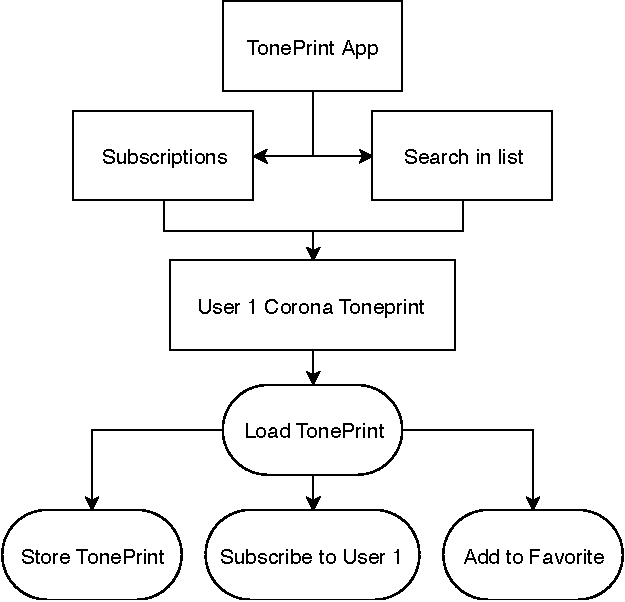
\includegraphics[width=0.9\textwidth]{2ICMM_new.pdf}
	\caption{The concept map for subject 2. The hand-drawn map is displayed in \autoref{fig:DrawnICMM2}.}
	\label{fig:ICMM2}
\end{figure}


\subsubsection{Subject 3}
\label{Subject3}
Subject 3 starts by opening the \textbf{TonePrint app} and gets a \textbf{notification} telling him that user 1, who he already \textbf{subscribes} to, has uploaded a new \textbf{Chorus TonePrint}. He tabs this notification, sending him directly to the specific \textbf{Chorus TonePrint site}, where he selects \textbf{save TonePrint}. From here he can then go to \textbf{user 1's profile} where he can check out other \textbf{TonePrints made by user 1}. He expects these to be sorted in a \textbf{logical order} such as \textbf{alphabetically} or something more fitting. \\
%
\begin{table}[H]
\begin{minipage}[b]{\linewidth}\centering
	\begin{tabular} {|l|l|l|} \hline
		\rowcolor{xGray25} \textbf{Content and Components} & \textbf{Actions} \\  \hline
		TonePrint app & pressing notification \\
		Notification system & Saving TonePrint \\
		Chorus TonePrints & pressing user 1's profile name \\
		Chorus TonePrint site &  \\
		User 1 profile &  \\
		User 1 TonePrint list &  \\
		Alphabetical sorting &  \\ \hline
	\end{tabular}
	\caption{The important content, components, and and actions mentioned by subject 3}
	\label{tab:Subject3ContentActions}
\end{minipage}
\end{table}
%
\begin{figure}[H]
	\centering
	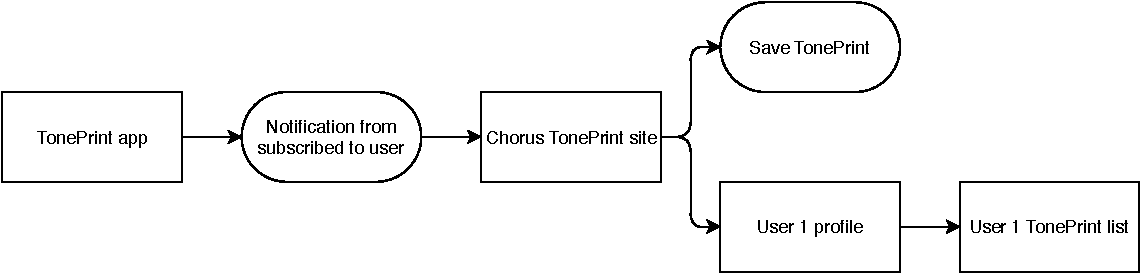
\includegraphics[width=0.9\textwidth]{3ICMM_new.pdf}
	\caption{The concept map for subject 3. The hand-drawn map is displayed in \autoref{fig:DrawnICMM3}.}
	\label{fig:ICMM3}
\end{figure}


\subsubsection{Subject 4}
\label{Subject4}
Subject 4 starts by opening the \textbf{TonePrint app} which he expects to have the same infrastructure as the current TonePrint app. He then navigates to \textbf{User TonePrints} where he expects to find all of his own TonePrints as well as an option called \textbf{cloud library}. By selecting this, he is redirected to where \textbf{all user TonePrints} are stored, and he wants find a TonePrint from a user that he already knows. He expects there to be a \textbf{filtering system} of some sort, and he chooses to \textbf{filter by product}, presenting him with a list of all \textbf{cloud based Corona TonePrints}. Subject 4 would then like to \textbf{search} for user 1, redirecting the list to the Corona TonePrints made by user 1. An alternative approach would be to just search for user 1 in the first place and be presented for all \textbf{user 1 TonePrints}. He considers this a more direct approach, as it only requires one action, but by using the current infrastructure of the TonePrint app, he would expect the filtering system to be a part of the solution. Subject 4 then enters \textbf{User 1’s profile}, where he is presented the TonePrints of user 1, although just the Corona types given the filtering system. He then clicks on a TonePrint with the intention of \textbf{trying it out in real time}, indicating that he wants to \textbf{transfer the TonePrint to his pedal}. If he then likes it, he can choose to \textbf{save it to his own library} and \textbf{highlight it as a favourite}. He wants an interface like the current TonePrint app, where he can \textbf{Save the TonePrint} and \textbf{Store it in pedal}. \\
%
\begin{table}[H]
\begin{minipage}[b]{\linewidth}\centering
	\begin{tabular} {|l|l|l|} \hline
		\rowcolor{xGray25} \textbf{Content and Components} & \textbf{Actions} \\  \hline
		TonePrint app & Selecting cloud library \\
		User TonePrints & Filter by product \\
		Cloud library & Searching for user 1 \\
		List of all user TonePrints & Clicking on a Corona TonePrint \\
		Filtering system & Trying TonePrint in real time \\
		Cloud based Corona TonePrints & Transfering TonePrint to pedal \\
		Search functionality & Saving TonePrint to his own library \\
		User 1 Corona TonePrints & Highlighting TonePrint as a favourite \\
		All user 1 TonePrints & Saving the TonePrint \\
		User 1 profile & Store TonePrint in pedal \\ \hline
	\end{tabular}
	\caption{The important content, components, and actions mentioned by subject 4}
	\label{tab:Subject4ContentActions}
\end{minipage}
\end{table}
%
\newpage
%
\begin{figure}[H]
	\centering
	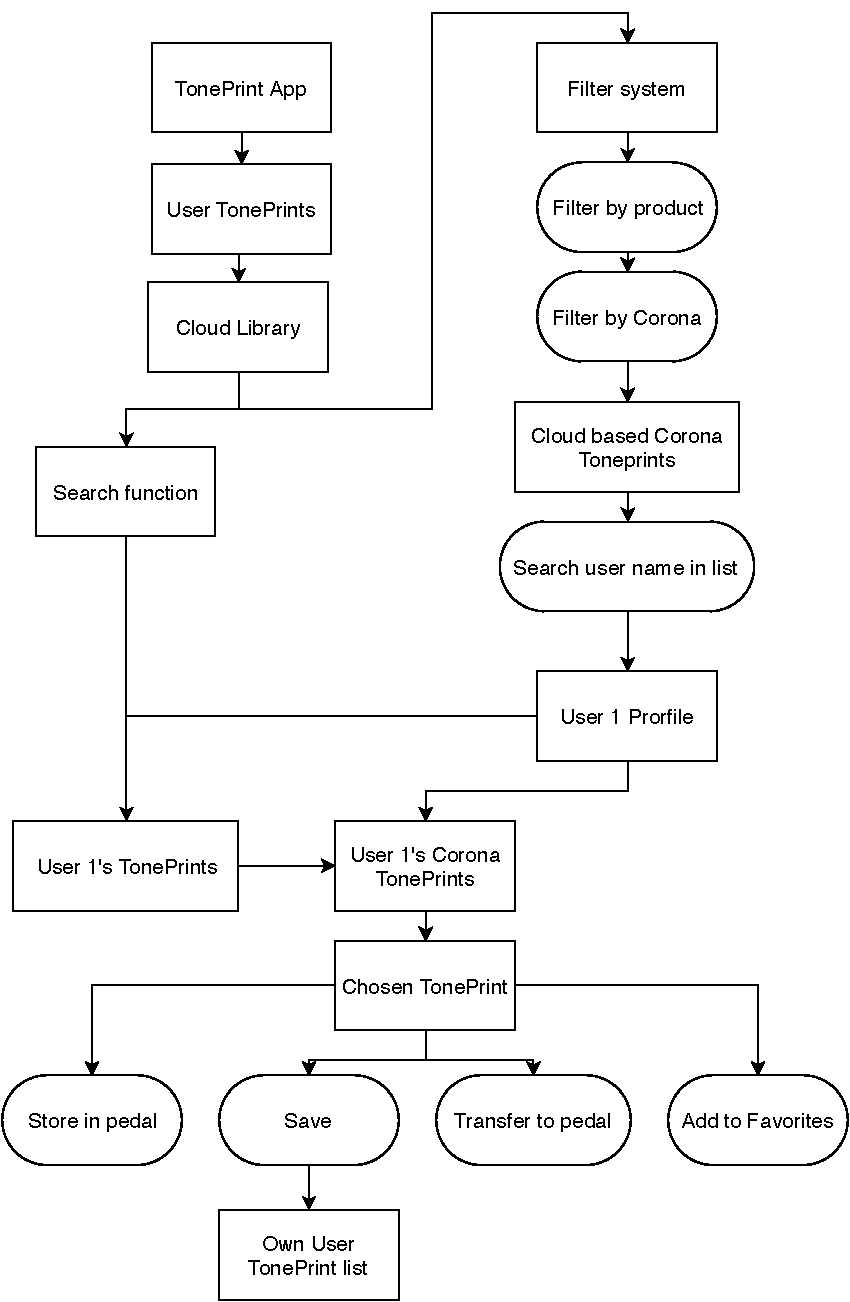
\includegraphics[width=\textwidth]{4ICMM_new.pdf}
	\caption{The concept map for subject 4. The hand-drawn map is displayed in \autoref{fig:DrawnICMM4}.}
	\label{fig:ICMM4}
\end{figure}


\subsubsection{Subject 5}
\label{Subject5}
Subject 5 starts by saying it needs to feel as familiar as possible, \textbf{similar to other apps} such as Youtube. Everyone uses these, and they tend to be somewhat similar. In the \textbf{TonePrint app} he therefore imagines a \textbf{magnifying glass icon} in the corner for \textbf{searching}, and he further proposes an \textbf{advanced search} for personalising the search. In either case, he proposes that it should work as a \textbf{meta search option}, where everything fitting to the search criteria within the system is presented to the user. In order to present this more organised, he proposes \textbf{different icons representing different content}. In the case of searching for user 1, the system would then provide a \textbf{suggested user: user 1}. By pressing this, the user is then redirected to all the \textbf{public content for user 1}, \textbf{sorted by products}. From here, he selects \textbf{Corona TonePrints} which unveils a \textbf{miniature view} of all user 1's TonePrints for this product, and when selecting one of these, the user is presented a site with all the \textbf{TonePrint details} and maybe a \textbf{picture} attached to the description. Should he just right click on it or hold a finger on it on the smartphone version, he would see a \textbf{context menu} with the options: \textbf{Beam}, \textbf{clone}, or \textbf{add to personal library}, allowing him to \textbf{edit it} or \textbf{highlight it as a favourite}. Finally, he describes a \textbf{history functionality} which allows him to \textbf{backtrack his actions}, much like in a web browser. As such, he will be able to find a TonePrint, even if he didn't highlight it as a favourite \\
%
\newpage
%
\begin{table}[H]
\begin{minipage}[b]{\linewidth}\centering
	\begin{tabular} {|l|l|l|} \hline
		\rowcolor{xGray25} \textbf{Content and Components} & \textbf{Actions} \\  \hline
		Similar to other apps & Pressing magnifying glass \\
		TonePrint app & Searching for user 1 \\
		Magnifying glass icon & Pressing suggest user: User 1 \\
		Search functionality & Selecting Corona TonePrints \\
		Advanced search & Selecting a specific TonePrint \\
		Meta search & Right clicking / holding a TonePrint \\
		Different icons for different content & adding to personal library \\
		Suggested user: User 1 & Further editing the TonePrint \\
		Public content for user 1 & Highlighting as favourite \\
		Corona TonePrints & Backtracking his actions \\
		Miniature view &  \\
		TonePrint details & \\
		Picture with the description & \\
		Context menu & \\
		Beaming option & \\
		Clone option & \\
		Add to personal library & \\
		Favourite option & \\
		Edit option & \\
		History functionality & \\ \hline
	\end{tabular}
	\caption{The important content, components, and actions mentioned by subject 5}
	\label{tab:Subject5ContentActions}
\end{minipage}
\end{table}
%
\begin{figure}[H]
	\centering
	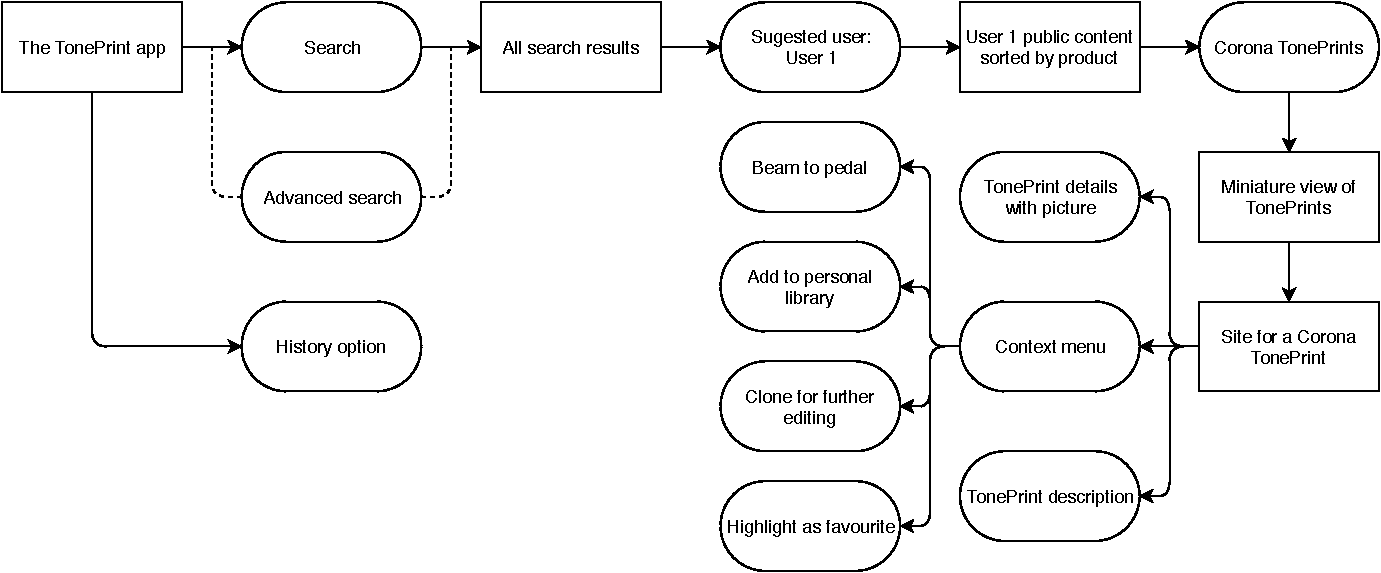
\includegraphics[width=\textwidth]{5ICMM_new.pdf}
	\caption{The concept map for subject 5. The hand-drawn map is displayed in \autoref{fig:DrawnICMM5}.}
	\label{fig:ICMM5}
\end{figure}
%
\newpage

\section{Reflecting on the task results}
\label{IndividualTaskReflection}
Before investigating the results of the group task, it seems fitting to first take a look at the results of the individual task in order to find common traits between the subjects. Had the workshop provided no major differences between them, then it would seem more or less straightforward, how the design of the information architecture should be approached, but this is not the case. It's also important to note that only 5 potential end-users participated as subjects in the workshop, and conducting more workshops with more subjects could just as well provide other results. All the subjects start the same way by opening the TonePrint app, with subject 4 even stating that he would expect to start from the current TonePrint app with the same infrastructure. They weren't instructed to approach the task on the basis of the current TonePrint app and the TonePrint community as one unit, but this might be due to bias from the task example. The route they then chose to reach the TonePrint made by user 1 turned out be rather different. Subject 1 and 4 propose they start by entering their own site of User TonePrints, where they have a tab giving them access to the public User TonePrints. subject 1 refers to this as \textit{friends} and \textit{community}, while subject 4 refers to it as \textit{cloud library}. For subject 2 and 5 it seems as the current app and community are completely unified, as they jump straight to a search functionality with subject 2 also proposing to enter a list of users that he already subscribes to. Subject 3 has the fastest route to the TonePrint of them all. He also proposes a subscription system, but in his version he receives a notification of a new TonePrint by user 1 that redirects him straight to it, skipping a lot of steps included by the other subjects.

Subject 1 and 4 then proposes a search functionality as well. Subject 4 first want to filter the vast amount of TonePrints by product, but both of them, as well as subject 2 and 5, wants to write "user1" and press the search result. This points towards that a search functionality should be included, even though it's not completely clear how the action itself and subsequent search results should be presented, and how advanced it should be. From the search there also seems to be some difference to where the subjects then expect to be redirected to. Subject 2, 4, and 5 expects to be taking directly to a list of all the TonePrints for user 1, with subject 5 referring to it as all the public content for user 1. Subject 1 expects to be taken to a profile for user 1, and this concept of a profile is present for more subjects, but he is the only one expecting to be taken to it at this point. In reality, all except subject 2 mentions a profile at some point during their presentation, and this would imply that profiles should in some way be a part of the TonePrint community. When reaching the correct TonePrint, the subjects generally have the same idea of what to do next. all subjects except subject 3 wants to highlight it as a favourite, and subject 1, 4, and 5 also wants to save or add it to their own TonePrint library while subject 2 and 4 talks about storing the TonePrint to the pedal. Subject 2 and 4 furthermore want to play with the TonePrint in real time before deciding on whether to save it or not. As final remarks, the subjects also proposed content for the TonePrint community such as backtracking, editing options for saved User TonePrints, and instructions for the TonePrints, including how to use them and their number of users.

\section{Group task result}
\label{GroupTaskResults}
For the second part of the workshop, the subjects were given a new task and told to produce one answer for it by reaching a common consensus instead of giving individual responses. As it has already been mentioned in the introduction for this chapter, subject 4 was excluded for this part, as he was considered a potential bias. Instead he observed the remaining subjects solving the task by his own request. The subjects were video recorded, as they engaged in a discussion of how to solve each step they found necessary in order to reach the end goal. The intention with this was to obtain a more reflective answer, as the subjects also needed to convince others of their proposes. \\

\noindent
The overall task was to upload a User TonePrint to the community, including the necessary meta data describing it, and from their point of view, the current way of setting parameters and naming a TonePrint should also be the way of doing it with the community integrated. The subjects then agreed that the need for descriptions and tags depended on whether the user in question wants to share the TonePrint with others. If the user only wants it for his own enjoyment, he should be able to simply skip the phase of describing and tagging it, but if he do wants to share it, the descriptions and tags are considered important. The distinction between a text description and tags was a heavily debated theme during the task, as the subjects considered the purpose of each somewhat similar. Both elements provide other users with info of the TonePrints in question, and one of the subjects even proposed including tags within the text description, maybe in the shape of hashtags, so they are clearly highlighted. The text description should nevertheless be something that the users write themselves, and one of the subjects also proposed to let the users include pictures with these.

The discussion then turned to how the design of the tagging system should be approached. They proposed that after writing a description for a TonePrint, the system should present a list of 'suggested tags'. These tags should be generated by the system itself, either from the parameter settings alone or also from the text description, and they should focus on different aspects of the TonePrint such as genre, effect type, craziness, etc. The intention with the 'craziness' tags would be to inform the user whether parameters have been set to extreme levels. It was also proposed that the suggested tags could be automatically applied by the system, while another subject wanted the suggested tags to appear in a drop-down menu. Finally, they also proposed the option of creating custom tags if the suggested ones weren't considered sufficient by the users.

After tagging, they then discussed how the sharing action should be done. The initial proposal was to simply highlight a TonePrint as 'public' but this wouldn't support the wish for also making more private sharing available. This lead to a discussion of how TonePrints could be shared with e.g. fellow band members by Facebook or mail, while not having it as a public TonePrint. one subject then proposed a solution similar to the smartphone app, snapchat, where it is possible to send content to either individual friends or groups of friends, although this probably isn't be the best analogy due to the content disappearing after being viewed. All this lead to three possible outcomes for sharing TonePrints. Firstly, the TonePrint could be kept private and therefore unavailable to other users of the community. The subjects referred to this as 'Unlisted' meaning it can only be found and accessed by the creator. Secondly, the creator could also choose to allow acces to a few people, if he decides to share it with them. Finally, he could just list it as public and allow access to anyone. In this scenario, the TonePrint would appear when searching matching criteria.

\subsection*{Presentation of group task}
\label{GroupTaskPresentation}
Just as with the individual task, the presentation of the concept map from the group task is also coded to highlight the important content, components, and actions. The group starts on the \textbf{page} of a \textbf{TonePrint} that they have just created. The first thing they do is \textbf{naming it} after which they are met by a \textbf{scheme} where they can \textbf{write a description} in their own words of TonePrint. They can also \textbf{upload a picture} of the band, the setup, or something else more descriptive. After this they are redirected to \textbf{suggested tags} based on \textbf{genre}, \textbf{effect type}, \textbf{sub-types} of the effect type, or a \textbf{craziness factor} if any parameters are set extremely high. After this, they are redirected to a \textbf{free tagging session}, where it is possible to include all the custom tags that they believe also describes the TonePrint. after this, they \textbf{save their changes} and are redirect to \textbf{privacy settings}. Here they can choose to make it \textbf{private}, so it's only available to oneself, they can set it as \textbf{unlisted}, making it private but shareable, or they can set it as \textbf{public}, making it visible to all. For both of the last two options, they can send it directly to their friends
%
\begin{table}[H]
\begin{minipage}[b]{\linewidth}\centering
	\begin{tabular} {|l|l|l|} \hline
		\rowcolor{xGray25} \textbf{Content and Components} & \textbf{Actions} \\  \hline
		TonePrint page & Naming it \\
		Description scheme & Writing a description \\
		Suggested tags & Uploading a picture \\
		Genre & Choosing suggested tags \\
		Effect type & Setting custom tags \\
		Sub-types & Saving changes \\
		Craziness factor & Choosing privacy settings \\
		Free tagging session & Spam my friends \\
		Privacy settings & \\
		Private & \\
		Unlisted & \\
		Public & \\ \hline
	\end{tabular}
	\caption{The important content, components, and and actions from the group task}
	\label{tab:GroupContentActions}
\end{minipage}
\end{table}
%
\newpage
%
\begin{figure}[H]
	\centering
	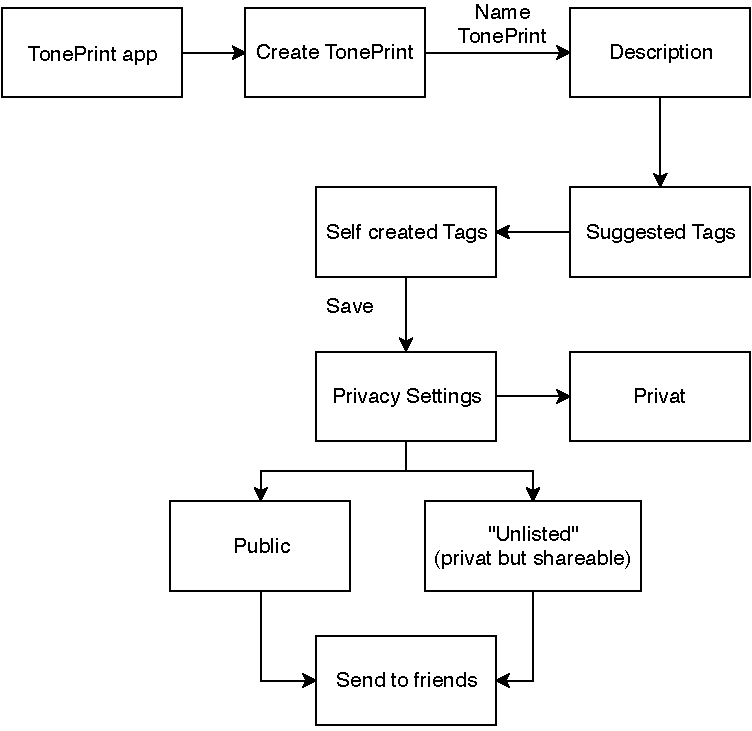
\includegraphics[width=\textwidth]{GruppeModel.pdf}
	\caption{The concept map for the group task. The hand-drawn map is displayed in \autoref{fig:GroupDraw}.}
	\label{fig:GroupConceptMap}
\end{figure}
%


%It's deemed problematic to use the described steps from \textcite{WEB:ConceptMapAnalysis} to create a ACSMM. This is because the task of the workshop was for the subjects to solve a task with a they have to build up as they go. This gives the users full control in regards to which features that exists in the system, how they works and when they wants to use them. This results in the subjects going different ways around the task and solving it in their won way. This is quite similar to some system in the real world which give you the option to reach a certain goal different ways. This however creates one big problem regarding, them only describing the part of the system, which they uses. This makes it very difficult to compare one persons ICMM with another, because they may have chosen different ways of solving the task and theirby having a minimal of similar concepts in common. This doesn't necessarily mean that the two subject disagree on how the system should work and their mental models might be similar towards the system. They just have chosen different approaches for the task, ehich means that they don't uses the same branches of the system. \\

